\thispagestyle{fancy}
\begin{center}
	\LARGE{\textbf{Potencia en un resistor}}
\end{center}
\section{Objetivos}
Al finalizar esta experiencia, usted estará capacitado para determinar la potencia en un resistor a partir de los valores de corriente y la tensión.
\section{Conocimientos previos}
La potencia en un resistor es el producto de la caída de tensión por la corriente. Normalmente se mide en Vatios (w).
\\
La ecuación para el cálculo de la potencia eléctrica es:
\begin{equation*}
	P=V*I
\end{equation*}
\\
\textbf{Donde:}
\begin{itemize}
	\item P = potencia en (w).
	\item V = tensión en (v).
	\item I = corriente en (A).
\end{itemize}
Podemos combinar la ecuación de la potencia y de la Ley de Ohm para obtener la relación entre la potencia y resistencia:
\begin{equation*}
	P = I^2 * R, P= \frac{V^2}{R}
\end{equation*}

Las lámparas brillan debido a la conversión de la energía eléctrica en energía lumínica. En esta experiencia, usted observará cómo la potencia es dada por el producto de la caída de tensión y la corriente.
\\
Se utilizarán dos lámparas de diferente resistencia para comparar la intensidad con la que brillan. Cuando las respectivas potencias sean iguales, el brillo será el mismo.
\section{Autoevaluación de entrada}
\begin{enumerate}
	\item Potencia es directamente proporcional al voltaje y a la corriente que circula por el circuito.
	\item La potencia en  un resistor es proporcional a voltaje y la intensidad de corriente.

\end{enumerate}
Usted puede empezar ahora la experiencia.
\section{Equipo}
Los siguientes equipos son necesarios para realizar esta experiencia:
\begin{enumerate}
	\item Módulo de experimentación.
	\item DMM (multímetro digital).
\end{enumerate}
\section{Procedimiento}
\begin{enumerate}
	\item Implemente el circuito de la  figura 1.
	\item Estudie el circuito de la figura 1, que contiene las lamparas $L_{1}$ y $L_{2}$:
	\begin{figure}[h]
		\centering
		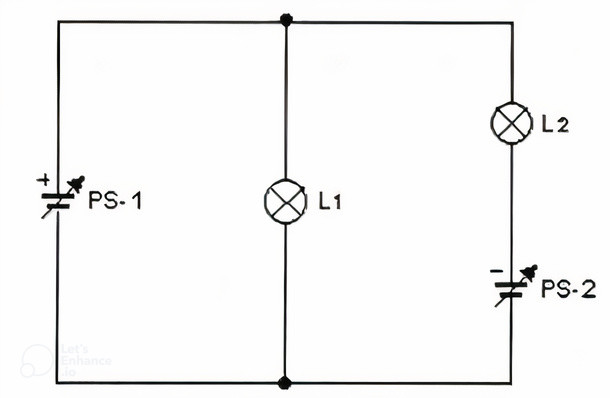
\includegraphics[scale=0.5]{imagenes/1}
		\caption{Circuito a armar}
	\end{figure}
	\item Lleve las tensiones de $PS-1$ y $PS-2$ hasta que el brillo de la lámpara $L_{2}$.
	\item Ahora aumente la tensión de salida de $PS-2$ hasta que el brillo de la lámpara $L_{2}$ iguales a la lámpara $L_{1}$.
	\\
	Mida la tensión en bornes de $L_{2}$ y la corriente que circula por dicha lámpara. 
	\\ Registre sus resultados: V igual a  e I igual a 
	\\ Calcule la potencia, registre el valor en el cuadro 1.
	\begin{table}[h]
		\centering
		\begin{tabular}{|c|c|c|}
			\hline
			\multicolumn{3}{c}{\textbf{Lampara 1}}\\ 
			\hline 
			\textbf{V (volt)}&\textbf{I (mA)}&\textbf{P (w)}\\
			\hline
			10 &2.60&260\\ 
			\hline
		\end{tabular}
		\caption{}
	\end{table}
	\item Ajuste la tensión en lámpara $L_{1}$  de acuerdo con los valores indicados en el cuadro 1. Ajuste la tensión de la lámpara $L_{2}$ hasta igualr los brillos de $L_{1}$ y $L_{2}$. En cada paso registre la corriente en $L_{1}$ y en $L_{2}$, y la tensión en $L_{2}$. Registre sus resultados en el cuadro 2.
	\begin{table}[h]
		\centering
		\begin{tabular}{|c|c|c|c|c|c|}
			\hline
			\multicolumn{3}{c}{\textbf{$L_{1}$}}&\multicolumn{3}{c}{\textbf{$L_{2}$}}\\
			\hline
			\textbf{V (volt)}&\textbf{I (mA)}&\textbf{P (mW)}&\textbf{V (volt)}&\textbf{I (mA)}&\textbf{P (mW)}\\
			\hline
			5&208&1040&5&208&1024\\
			\hline
			6&250&1500&6&250&1500\\
			\hline
			7&292&2044&7&292&2044\\
			\hline
			8&333&2664&8&333&2664\\
			\hline
			9&375&3375&9&375&3375\\
			\hline
			10&417&4170&10&417&4170\\
			\hline
		\end{tabular}
		\caption{}
	\end{table}
	\item Utilizando la ecuación $P=V*I$, calcule la potencia en cada lámpara para cada ajuste de tensión. Registre los valores calculados en el cuadro 2 modifica.
\end{enumerate}
\section{Autoevaluación}
\begin{enumerate}
	\item El método de comparar la intensidad del brillo de dos lámparas con el objeto de determinar si sus potencias son iguales es verdadero puesto que a mayor voltaje y corriente mayor es  el brillo.
	\item Cuando la tensión en dos lámparas es la misma, brillarán con la misma intensidad y también la potencia va aumentar.
\end{enumerate}
\section{Conclusión}
En este laboratorio se llego a experimentar  que la iluminación de las lamparas van ir a acorde de como va subiendo mientras que el voltaje va subiendo y la corriente en el circuito va aumentando. Con este experimento se llego ver que la potencia es directamente proporcional al voltaje y a la intensidad de corriente.
\section{Anexo}
\begin{figure}[h]
	\begin{minipage}{0.35\textwidth}
		\centering
		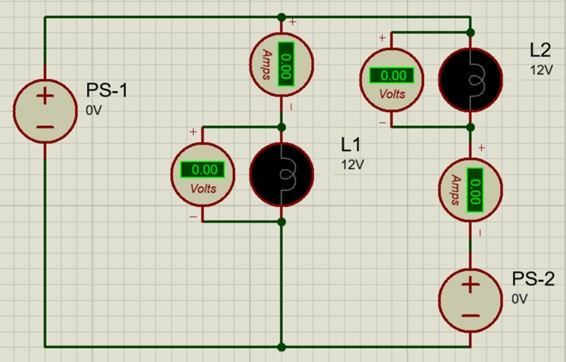
\includegraphics[width=0.8\linewidth]{imagenes/3}
		
	\end{minipage}%
	\begin{minipage}{0.35\textwidth}
		\centering
		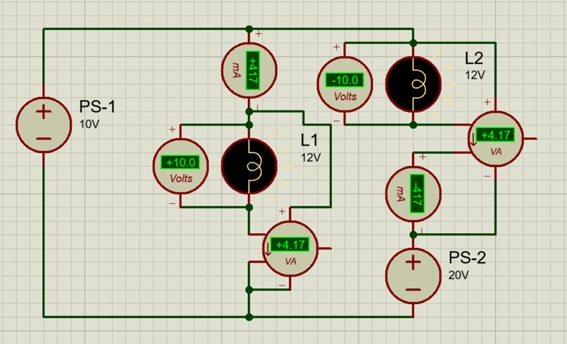
\includegraphics[width=0.8\linewidth]{imagenes/4}
		
	\end{minipage}
\end{figure}

\begin{figure}[h]
	\begin{minipage}{0.35\textwidth}
		\centering
		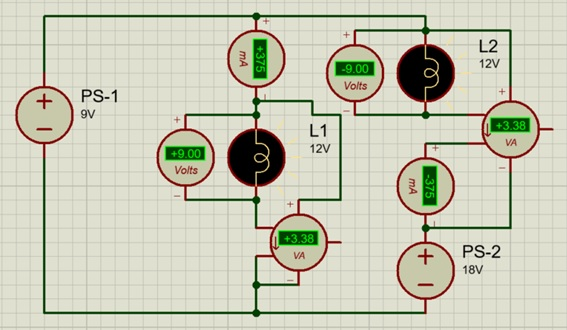
\includegraphics[width=0.8\linewidth]{imagenes/5}
		
	\end{minipage}%
	\begin{minipage}{0.35\textwidth}
		\centering
		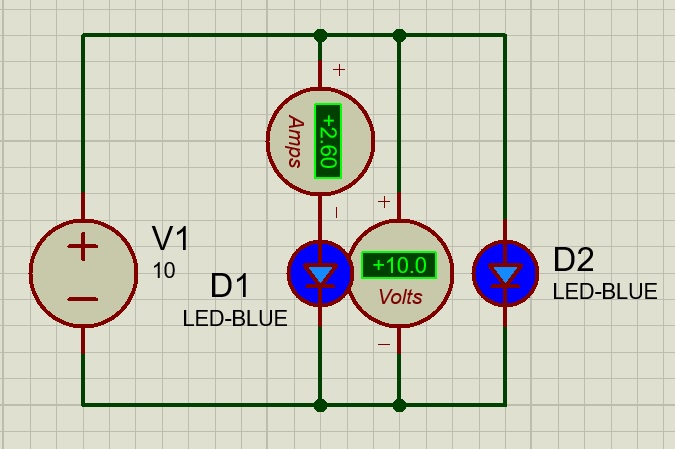
\includegraphics[width=0.8\linewidth]{imagenes/7}
		
	\end{minipage}
\end{figure}
